% !TEX TS-program = xelatex
% !TEX encoding = UTF-8 Unicode
% 都灵理工学院 Politecnico of Torino
% 模板维护者 Claudio Fiandrino
% 官网 https://github.com/cfiandra/Beamer2Thesis
\documentclass{beamer}
\usetheme[titlepagelogo=logo,
		  language=english,
		  bullet=triangle,
		  color=green,   % red green blue
		]{TorinoTh}
\usepackage[beamer,customcolors]{hf-tikz}
\hfsetfillcolor{alerted text.fg!10}
\hfsetbordercolor{alerted text.fg}
\usepackage{xeCJK}
\usepackage{natbib} % 参考文献
% \setsansfont{Ubuntu}
% \setsansfont{Fira Sans}
\setsansfont{Roboto}

\defaultfontfeatures{Mapping=tex-text}
\setCJKmainfont[BoldFont=Noto Sans CJK SC, ItalicFont=Adobe Kaiti Std]{Source Han Serif SC}
\setCJKmonofont[Scale=0.9]{Adobe Kaiti Std}
\setCJKfamilyfont{song}[BoldFont=Noto Sans CJK SC]{Source Han Serif SC}
\setCJKfamilyfont{sf}[BoldFont=Noto Sans CJK SC]{Noto Sans CJK SC}

\renewcommand\contentsname{目录}
\renewcommand\listfigurename{插图列表}
\renewcommand\listtablename{表格列表}
\renewcommand\refname{参考文献}
\renewcommand\indexname{索引}
\renewcommand\figurename{图}
\renewcommand\tablename{表}
\renewcommand\partname{部分}
\renewcommand\appendixname{附录}
\renewcommand\abstractname{摘要}


\graphicspath{{figures/}} % 图片路径

\author{黄湘云} % 答辩人
\rel{李再兴} % 导师
\title{空间广义线性混合模型及其在预测流行病中的应用}
\ateneo{硕士论文答辩}
\date{\today}
\keywords{SGLMM}
\subject{硕士论文答辩}

\begin{document}
\titlepageframe

\begin{tframe}

\textbf{Outline}
\begin{enumerate}
  \item Introduction (Motivations and goals)
  \item Literature reviews  
  \item Geostatistical model (SGLMM)
  \item Computing details and simulations
  \item Real data analysis (Applications)
  \item Discussion
\end{enumerate}
\end{tframe}

\section{Intro}

\begin{tframe}
\begin{figure}
\centering
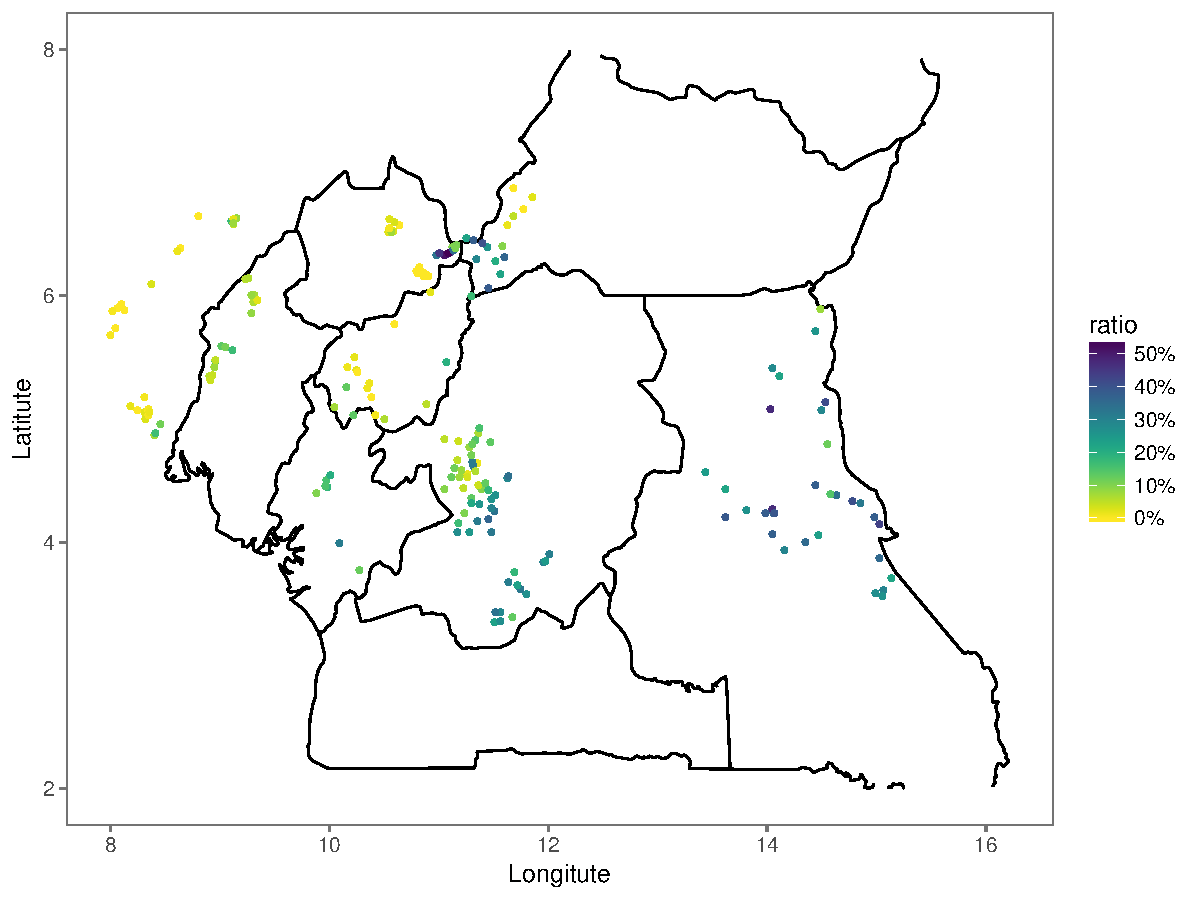
\includegraphics[width=.8\textwidth]{demo01}
\end{figure}
\end{tframe}

\begin{tframe}
\begin{figure}
\centering
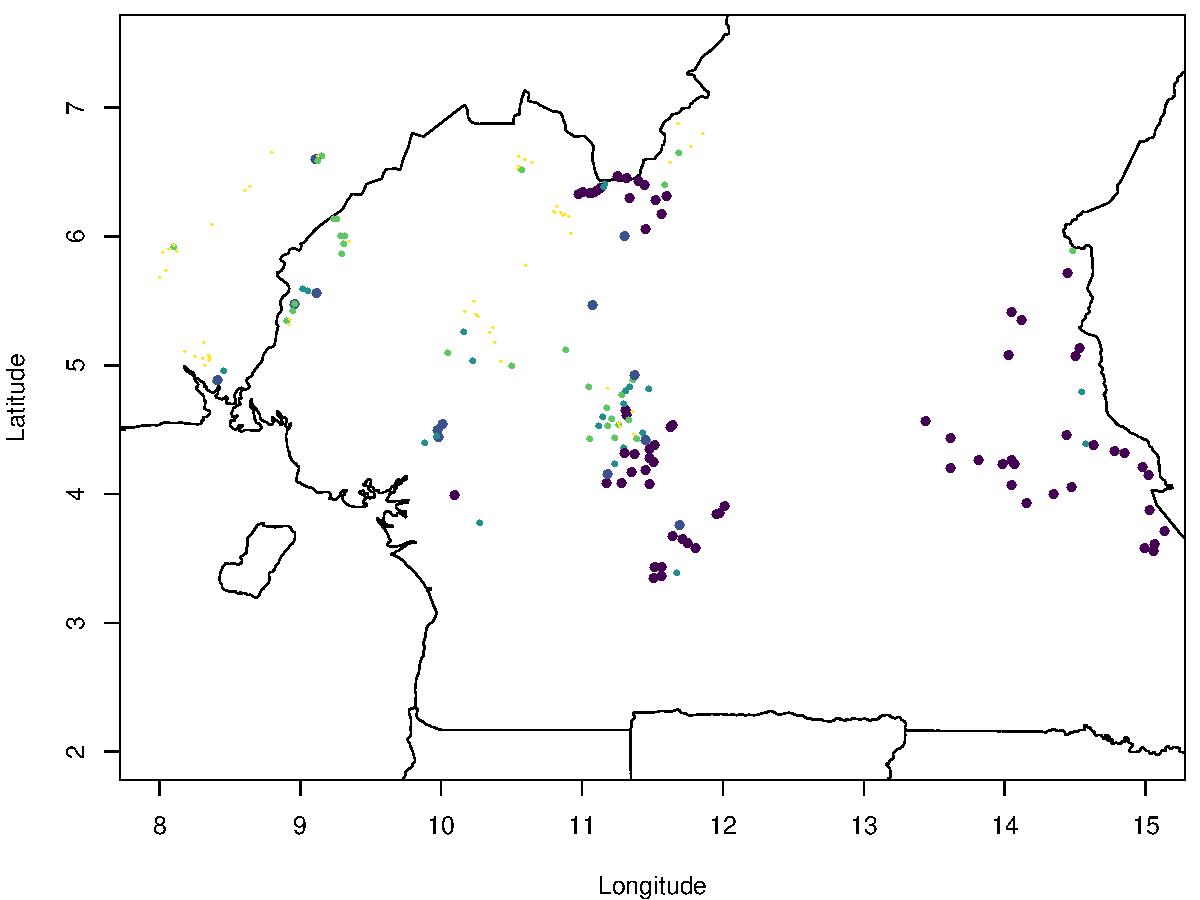
\includegraphics[width=.8\textwidth]{demo010}
\end{figure}
\end{tframe}

\begin{tframe}
\begin{figure}
\centering
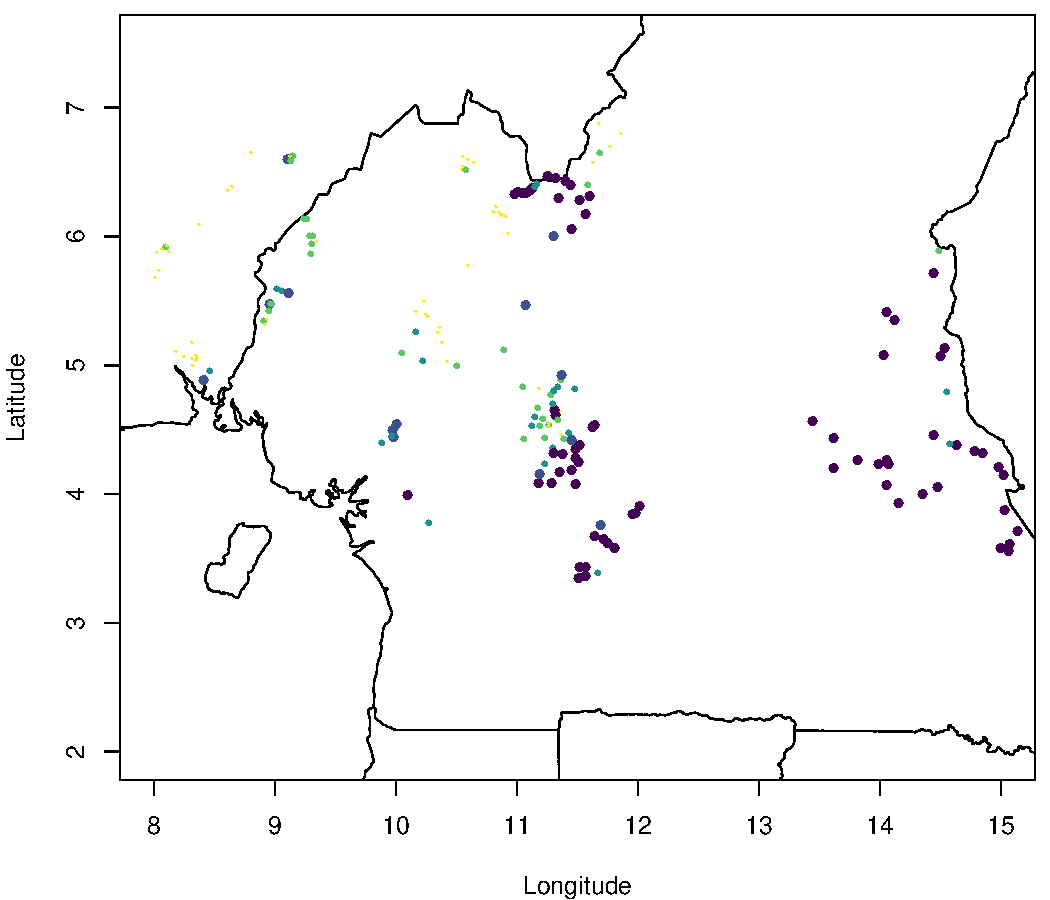
\includegraphics[width=.8\textwidth]{demo011}
\end{figure}
\end{tframe}

\begin{tframe}
\begin{figure}
\centering
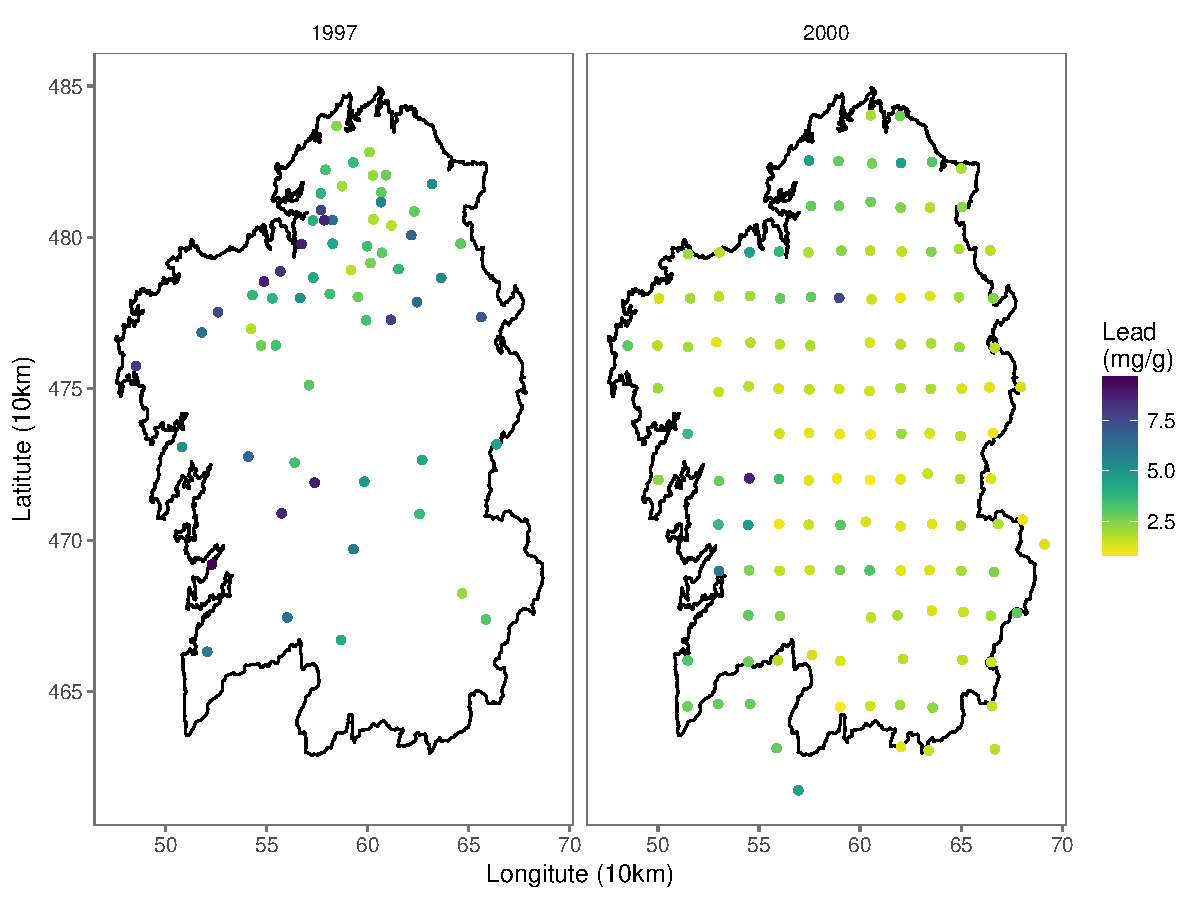
\includegraphics[width=.8\textwidth]{demo03}
\end{figure}
\end{tframe}



\section{refs}

\begin{frame}[allowframebreaks]
\frametitle{Frameworks, Packages and Softwares}

\begin{description}
\item[\textbf{R:}] geoR geoRglm spatial PrevMap \\
\citet{R-geoR,R-geoRglm,R-spatial,Giorgi2016}

\item[\textbf{Stan:}] Stan \footnote{\scriptsize \url{http://mc-stan.org/} }  
interfaces with R (RStan) ,Python (PyStan) , MATLAB (MatlabStan) 
and  more \\ \citet{Stan2015,Stan2017}

\item[\textbf{PyMC3:}] Probabilistic programming in Python using PyMC3 \\ \citet{Salvatier2016}

\item[\textbf{JAGS:}] \textbf{J}ust \textbf{A}nother \textbf{G}ibbs \textbf{S}ampler \footnote{\scriptsize \url{https://en.wikipedia.org/wiki/Just_another_Gibbs_sampler}} \\
Bayesian hierarchical models using Markov chain Monte Carlo (MCMC)
\item[\textbf{BUGS:}] \textbf{B}ayesian inference \textbf{U}sing \textbf{G}ibbs \textbf{S}ampling ,
such as winBUGS, OpenBUGS 
\item[\textbf{R-INLA:}] \textbf{I}ntegrated \textbf{N}ested \textbf{L}aplace \textbf{A}pproximations \\
\citet{Rue2009,R-INLA,Rue2017arXiv}
\end{description}


\end{frame}



\begin{frame}[allowframebreaks]
\bibliographystyle{authordate1}
\bibliography{R-GLMM-pkgs}
\end{frame}

\end{document} 


